% Created by tikzDevice version 0.12.3.1 on 2023-05-03 19:55:08
% !TEX encoding = UTF-8 Unicode
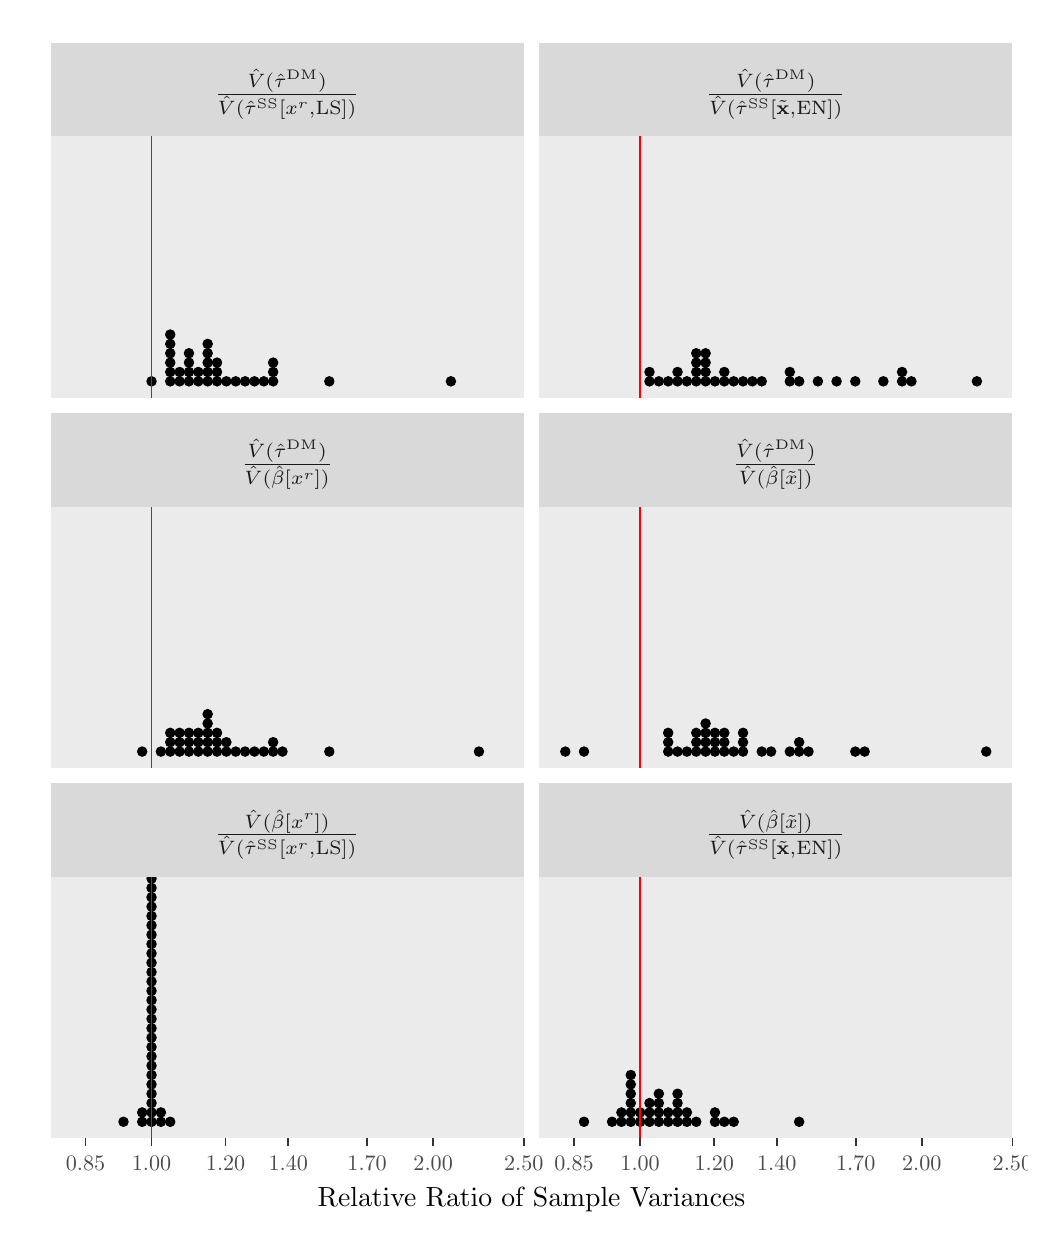
\begin{tikzpicture}[x=1pt,y=1pt]
\definecolor{fillColor}{RGB}{255,255,255}
\path[use as bounding box,fill=fillColor,fill opacity=0.00] (0,0) rectangle (361.35,433.62);
\begin{scope}
\path[clip] (  0.00,  0.00) rectangle (361.35,433.62);
\definecolor{drawColor}{RGB}{255,255,255}
\definecolor{fillColor}{RGB}{255,255,255}

\path[draw=drawColor,line width= 0.6pt,line join=round,line cap=round,fill=fillColor] (  0.00,  0.00) rectangle (361.35,433.62);
\end{scope}
\begin{scope}
\path[clip] (  8.25,299.84) rectangle (179.30,394.32);
\definecolor{fillColor}{gray}{0.92}

\path[fill=fillColor] (  8.25,299.84) rectangle (179.30,394.32);
\definecolor{drawColor}{RGB}{0,0,0}
\definecolor{fillColor}{RGB}{0,0,0}

\path[draw=drawColor,line width= 0.4pt,line join=round,fill=fillColor] ( 44.76,305.82) circle (  1.69);

\path[draw=drawColor,line width= 0.4pt,line join=round,fill=fillColor] ( 51.52,305.82) circle (  1.69);

\path[draw=drawColor,line width= 0.4pt,line join=round,fill=fillColor] ( 51.52,309.20) circle (  1.69);

\path[draw=drawColor,line width= 0.4pt,line join=round,fill=fillColor] ( 51.52,312.58) circle (  1.69);

\path[draw=drawColor,line width= 0.4pt,line join=round,fill=fillColor] ( 51.52,315.96) circle (  1.69);

\path[draw=drawColor,line width= 0.4pt,line join=round,fill=fillColor] ( 51.52,319.35) circle (  1.69);

\path[draw=drawColor,line width= 0.4pt,line join=round,fill=fillColor] ( 51.52,322.73) circle (  1.69);

\path[draw=drawColor,line width= 0.4pt,line join=round,fill=fillColor] ( 54.90,305.82) circle (  1.69);

\path[draw=drawColor,line width= 0.4pt,line join=round,fill=fillColor] ( 54.90,309.20) circle (  1.69);

\path[draw=drawColor,line width= 0.4pt,line join=round,fill=fillColor] ( 58.28,305.82) circle (  1.69);

\path[draw=drawColor,line width= 0.4pt,line join=round,fill=fillColor] ( 58.28,309.20) circle (  1.69);

\path[draw=drawColor,line width= 0.4pt,line join=round,fill=fillColor] ( 58.28,312.58) circle (  1.69);

\path[draw=drawColor,line width= 0.4pt,line join=round,fill=fillColor] ( 58.28,315.96) circle (  1.69);

\path[draw=drawColor,line width= 0.4pt,line join=round,fill=fillColor] ( 61.66,305.82) circle (  1.69);

\path[draw=drawColor,line width= 0.4pt,line join=round,fill=fillColor] ( 61.66,309.20) circle (  1.69);

\path[draw=drawColor,line width= 0.4pt,line join=round,fill=fillColor] ( 65.04,305.82) circle (  1.69);

\path[draw=drawColor,line width= 0.4pt,line join=round,fill=fillColor] ( 65.04,309.20) circle (  1.69);

\path[draw=drawColor,line width= 0.4pt,line join=round,fill=fillColor] ( 65.04,312.58) circle (  1.69);

\path[draw=drawColor,line width= 0.4pt,line join=round,fill=fillColor] ( 65.04,315.96) circle (  1.69);

\path[draw=drawColor,line width= 0.4pt,line join=round,fill=fillColor] ( 65.04,319.35) circle (  1.69);

\path[draw=drawColor,line width= 0.4pt,line join=round,fill=fillColor] ( 68.42,305.82) circle (  1.69);

\path[draw=drawColor,line width= 0.4pt,line join=round,fill=fillColor] ( 68.42,309.20) circle (  1.69);

\path[draw=drawColor,line width= 0.4pt,line join=round,fill=fillColor] ( 68.42,312.58) circle (  1.69);

\path[draw=drawColor,line width= 0.4pt,line join=round,fill=fillColor] ( 71.80,305.82) circle (  1.69);

\path[draw=drawColor,line width= 0.4pt,line join=round,fill=fillColor] ( 75.18,305.82) circle (  1.69);

\path[draw=drawColor,line width= 0.4pt,line join=round,fill=fillColor] ( 78.56,305.82) circle (  1.69);

\path[draw=drawColor,line width= 0.4pt,line join=round,fill=fillColor] ( 81.94,305.82) circle (  1.69);

\path[draw=drawColor,line width= 0.4pt,line join=round,fill=fillColor] ( 85.32,305.82) circle (  1.69);

\path[draw=drawColor,line width= 0.4pt,line join=round,fill=fillColor] ( 88.70,305.82) circle (  1.69);

\path[draw=drawColor,line width= 0.4pt,line join=round,fill=fillColor] ( 88.70,309.20) circle (  1.69);

\path[draw=drawColor,line width= 0.4pt,line join=round,fill=fillColor] ( 88.70,312.58) circle (  1.69);

\path[draw=drawColor,line width= 0.4pt,line join=round,fill=fillColor] (108.99,305.82) circle (  1.69);

\path[draw=drawColor,line width= 0.4pt,line join=round,fill=fillColor] (152.93,305.82) circle (  1.69);
\definecolor{drawColor}{RGB}{255,0,0}

\path[draw=drawColor,line width= 0.6pt,line join=round] ( 44.76,299.84) -- ( 44.76,394.32);
\end{scope}
\begin{scope}
\path[clip] (  8.25,166.06) rectangle (179.30,260.54);
\definecolor{fillColor}{gray}{0.92}

\path[fill=fillColor] (  8.25,166.06) rectangle (179.30,260.54);
\definecolor{drawColor}{RGB}{0,0,0}
\definecolor{fillColor}{RGB}{0,0,0}

\path[draw=drawColor,line width= 0.4pt,line join=round,fill=fillColor] ( 41.38,172.04) circle (  1.69);

\path[draw=drawColor,line width= 0.4pt,line join=round,fill=fillColor] ( 48.14,172.04) circle (  1.69);

\path[draw=drawColor,line width= 0.4pt,line join=round,fill=fillColor] ( 51.52,172.04) circle (  1.69);

\path[draw=drawColor,line width= 0.4pt,line join=round,fill=fillColor] ( 51.52,175.42) circle (  1.69);

\path[draw=drawColor,line width= 0.4pt,line join=round,fill=fillColor] ( 51.52,178.80) circle (  1.69);

\path[draw=drawColor,line width= 0.4pt,line join=round,fill=fillColor] ( 54.90,172.04) circle (  1.69);

\path[draw=drawColor,line width= 0.4pt,line join=round,fill=fillColor] ( 54.90,175.42) circle (  1.69);

\path[draw=drawColor,line width= 0.4pt,line join=round,fill=fillColor] ( 54.90,178.80) circle (  1.69);

\path[draw=drawColor,line width= 0.4pt,line join=round,fill=fillColor] ( 58.28,172.04) circle (  1.69);

\path[draw=drawColor,line width= 0.4pt,line join=round,fill=fillColor] ( 58.28,175.42) circle (  1.69);

\path[draw=drawColor,line width= 0.4pt,line join=round,fill=fillColor] ( 58.28,178.80) circle (  1.69);

\path[draw=drawColor,line width= 0.4pt,line join=round,fill=fillColor] ( 61.66,172.04) circle (  1.69);

\path[draw=drawColor,line width= 0.4pt,line join=round,fill=fillColor] ( 61.66,175.42) circle (  1.69);

\path[draw=drawColor,line width= 0.4pt,line join=round,fill=fillColor] ( 61.66,178.80) circle (  1.69);

\path[draw=drawColor,line width= 0.4pt,line join=round,fill=fillColor] ( 65.04,172.04) circle (  1.69);

\path[draw=drawColor,line width= 0.4pt,line join=round,fill=fillColor] ( 65.04,175.42) circle (  1.69);

\path[draw=drawColor,line width= 0.4pt,line join=round,fill=fillColor] ( 65.04,178.80) circle (  1.69);

\path[draw=drawColor,line width= 0.4pt,line join=round,fill=fillColor] ( 65.04,182.18) circle (  1.69);

\path[draw=drawColor,line width= 0.4pt,line join=round,fill=fillColor] ( 65.04,185.56) circle (  1.69);

\path[draw=drawColor,line width= 0.4pt,line join=round,fill=fillColor] ( 68.42,172.04) circle (  1.69);

\path[draw=drawColor,line width= 0.4pt,line join=round,fill=fillColor] ( 68.42,175.42) circle (  1.69);

\path[draw=drawColor,line width= 0.4pt,line join=round,fill=fillColor] ( 68.42,178.80) circle (  1.69);

\path[draw=drawColor,line width= 0.4pt,line join=round,fill=fillColor] ( 71.80,172.04) circle (  1.69);

\path[draw=drawColor,line width= 0.4pt,line join=round,fill=fillColor] ( 71.80,175.42) circle (  1.69);

\path[draw=drawColor,line width= 0.4pt,line join=round,fill=fillColor] ( 75.18,172.04) circle (  1.69);

\path[draw=drawColor,line width= 0.4pt,line join=round,fill=fillColor] ( 78.56,172.04) circle (  1.69);

\path[draw=drawColor,line width= 0.4pt,line join=round,fill=fillColor] ( 81.94,172.04) circle (  1.69);

\path[draw=drawColor,line width= 0.4pt,line join=round,fill=fillColor] ( 85.32,172.04) circle (  1.69);

\path[draw=drawColor,line width= 0.4pt,line join=round,fill=fillColor] ( 88.70,172.04) circle (  1.69);

\path[draw=drawColor,line width= 0.4pt,line join=round,fill=fillColor] ( 88.70,175.42) circle (  1.69);

\path[draw=drawColor,line width= 0.4pt,line join=round,fill=fillColor] ( 92.08,172.04) circle (  1.69);

\path[draw=drawColor,line width= 0.4pt,line join=round,fill=fillColor] (108.99,172.04) circle (  1.69);

\path[draw=drawColor,line width= 0.4pt,line join=round,fill=fillColor] (163.07,172.04) circle (  1.69);
\definecolor{drawColor}{RGB}{255,0,0}

\path[draw=drawColor,line width= 0.6pt,line join=round] ( 44.76,166.06) -- ( 44.76,260.54);
\end{scope}
\begin{scope}
\path[clip] (  8.25, 32.28) rectangle (179.30,126.76);
\definecolor{fillColor}{gray}{0.92}

\path[fill=fillColor] (  8.25, 32.28) rectangle (179.30,126.76);
\definecolor{drawColor}{RGB}{0,0,0}
\definecolor{fillColor}{RGB}{0,0,0}

\path[draw=drawColor,line width= 0.4pt,line join=round,fill=fillColor] ( 34.62, 38.26) circle (  1.69);

\path[draw=drawColor,line width= 0.4pt,line join=round,fill=fillColor] ( 41.38, 38.26) circle (  1.69);

\path[draw=drawColor,line width= 0.4pt,line join=round,fill=fillColor] ( 41.38, 41.64) circle (  1.69);

\path[draw=drawColor,line width= 0.4pt,line join=round,fill=fillColor] ( 44.76, 38.26) circle (  1.69);

\path[draw=drawColor,line width= 0.4pt,line join=round,fill=fillColor] ( 44.76, 41.64) circle (  1.69);

\path[draw=drawColor,line width= 0.4pt,line join=round,fill=fillColor] ( 44.76, 45.02) circle (  1.69);

\path[draw=drawColor,line width= 0.4pt,line join=round,fill=fillColor] ( 44.76, 48.40) circle (  1.69);

\path[draw=drawColor,line width= 0.4pt,line join=round,fill=fillColor] ( 44.76, 51.78) circle (  1.69);

\path[draw=drawColor,line width= 0.4pt,line join=round,fill=fillColor] ( 44.76, 55.16) circle (  1.69);

\path[draw=drawColor,line width= 0.4pt,line join=round,fill=fillColor] ( 44.76, 58.54) circle (  1.69);

\path[draw=drawColor,line width= 0.4pt,line join=round,fill=fillColor] ( 44.76, 61.92) circle (  1.69);

\path[draw=drawColor,line width= 0.4pt,line join=round,fill=fillColor] ( 44.76, 65.30) circle (  1.69);

\path[draw=drawColor,line width= 0.4pt,line join=round,fill=fillColor] ( 44.76, 68.68) circle (  1.69);

\path[draw=drawColor,line width= 0.4pt,line join=round,fill=fillColor] ( 44.76, 72.06) circle (  1.69);

\path[draw=drawColor,line width= 0.4pt,line join=round,fill=fillColor] ( 44.76, 75.45) circle (  1.69);

\path[draw=drawColor,line width= 0.4pt,line join=round,fill=fillColor] ( 44.76, 78.83) circle (  1.69);

\path[draw=drawColor,line width= 0.4pt,line join=round,fill=fillColor] ( 44.76, 82.21) circle (  1.69);

\path[draw=drawColor,line width= 0.4pt,line join=round,fill=fillColor] ( 44.76, 85.59) circle (  1.69);

\path[draw=drawColor,line width= 0.4pt,line join=round,fill=fillColor] ( 44.76, 88.97) circle (  1.69);

\path[draw=drawColor,line width= 0.4pt,line join=round,fill=fillColor] ( 44.76, 92.35) circle (  1.69);

\path[draw=drawColor,line width= 0.4pt,line join=round,fill=fillColor] ( 44.76, 95.73) circle (  1.69);

\path[draw=drawColor,line width= 0.4pt,line join=round,fill=fillColor] ( 44.76, 99.11) circle (  1.69);

\path[draw=drawColor,line width= 0.4pt,line join=round,fill=fillColor] ( 44.76,102.49) circle (  1.69);

\path[draw=drawColor,line width= 0.4pt,line join=round,fill=fillColor] ( 44.76,105.87) circle (  1.69);

\path[draw=drawColor,line width= 0.4pt,line join=round,fill=fillColor] ( 44.76,109.25) circle (  1.69);

\path[draw=drawColor,line width= 0.4pt,line join=round,fill=fillColor] ( 44.76,112.63) circle (  1.69);

\path[draw=drawColor,line width= 0.4pt,line join=round,fill=fillColor] ( 44.76,116.01) circle (  1.69);

\path[draw=drawColor,line width= 0.4pt,line join=round,fill=fillColor] ( 44.76,119.39) circle (  1.69);

\path[draw=drawColor,line width= 0.4pt,line join=round,fill=fillColor] ( 44.76,122.77) circle (  1.69);

\path[draw=drawColor,line width= 0.4pt,line join=round,fill=fillColor] ( 44.76,126.15) circle (  1.69);

\path[draw=drawColor,line width= 0.4pt,line join=round,fill=fillColor] ( 48.14, 38.26) circle (  1.69);

\path[draw=drawColor,line width= 0.4pt,line join=round,fill=fillColor] ( 48.14, 41.64) circle (  1.69);

\path[draw=drawColor,line width= 0.4pt,line join=round,fill=fillColor] ( 51.52, 38.26) circle (  1.69);
\definecolor{drawColor}{RGB}{255,0,0}

\path[draw=drawColor,line width= 0.6pt,line join=round] ( 44.76, 32.28) -- ( 44.76,126.76);
\end{scope}
\begin{scope}
\path[clip] (184.80,299.84) rectangle (355.85,394.32);
\definecolor{fillColor}{gray}{0.92}

\path[fill=fillColor] (184.80,299.84) rectangle (355.85,394.32);
\definecolor{drawColor}{RGB}{0,0,0}
\definecolor{fillColor}{RGB}{0,0,0}

\path[draw=drawColor,line width= 0.4pt,line join=round,fill=fillColor] (224.69,305.82) circle (  1.69);

\path[draw=drawColor,line width= 0.4pt,line join=round,fill=fillColor] (224.69,309.20) circle (  1.69);

\path[draw=drawColor,line width= 0.4pt,line join=round,fill=fillColor] (228.07,305.82) circle (  1.69);

\path[draw=drawColor,line width= 0.4pt,line join=round,fill=fillColor] (231.45,305.82) circle (  1.69);

\path[draw=drawColor,line width= 0.4pt,line join=round,fill=fillColor] (234.83,305.82) circle (  1.69);

\path[draw=drawColor,line width= 0.4pt,line join=round,fill=fillColor] (234.83,309.20) circle (  1.69);

\path[draw=drawColor,line width= 0.4pt,line join=round,fill=fillColor] (238.21,305.82) circle (  1.69);

\path[draw=drawColor,line width= 0.4pt,line join=round,fill=fillColor] (241.59,305.82) circle (  1.69);

\path[draw=drawColor,line width= 0.4pt,line join=round,fill=fillColor] (241.59,309.20) circle (  1.69);

\path[draw=drawColor,line width= 0.4pt,line join=round,fill=fillColor] (241.59,312.58) circle (  1.69);

\path[draw=drawColor,line width= 0.4pt,line join=round,fill=fillColor] (241.59,315.96) circle (  1.69);

\path[draw=drawColor,line width= 0.4pt,line join=round,fill=fillColor] (244.97,305.82) circle (  1.69);

\path[draw=drawColor,line width= 0.4pt,line join=round,fill=fillColor] (244.97,309.20) circle (  1.69);

\path[draw=drawColor,line width= 0.4pt,line join=round,fill=fillColor] (244.97,312.58) circle (  1.69);

\path[draw=drawColor,line width= 0.4pt,line join=round,fill=fillColor] (244.97,315.96) circle (  1.69);

\path[draw=drawColor,line width= 0.4pt,line join=round,fill=fillColor] (248.35,305.82) circle (  1.69);

\path[draw=drawColor,line width= 0.4pt,line join=round,fill=fillColor] (251.73,305.82) circle (  1.69);

\path[draw=drawColor,line width= 0.4pt,line join=round,fill=fillColor] (251.73,309.20) circle (  1.69);

\path[draw=drawColor,line width= 0.4pt,line join=round,fill=fillColor] (255.11,305.82) circle (  1.69);

\path[draw=drawColor,line width= 0.4pt,line join=round,fill=fillColor] (258.49,305.82) circle (  1.69);

\path[draw=drawColor,line width= 0.4pt,line join=round,fill=fillColor] (261.87,305.82) circle (  1.69);

\path[draw=drawColor,line width= 0.4pt,line join=round,fill=fillColor] (265.25,305.82) circle (  1.69);

\path[draw=drawColor,line width= 0.4pt,line join=round,fill=fillColor] (275.40,305.82) circle (  1.69);

\path[draw=drawColor,line width= 0.4pt,line join=round,fill=fillColor] (275.40,309.20) circle (  1.69);

\path[draw=drawColor,line width= 0.4pt,line join=round,fill=fillColor] (278.78,305.82) circle (  1.69);

\path[draw=drawColor,line width= 0.4pt,line join=round,fill=fillColor] (285.54,305.82) circle (  1.69);

\path[draw=drawColor,line width= 0.4pt,line join=round,fill=fillColor] (292.30,305.82) circle (  1.69);

\path[draw=drawColor,line width= 0.4pt,line join=round,fill=fillColor] (299.06,305.82) circle (  1.69);

\path[draw=drawColor,line width= 0.4pt,line join=round,fill=fillColor] (309.20,305.82) circle (  1.69);

\path[draw=drawColor,line width= 0.4pt,line join=round,fill=fillColor] (315.96,305.82) circle (  1.69);

\path[draw=drawColor,line width= 0.4pt,line join=round,fill=fillColor] (315.96,309.20) circle (  1.69);

\path[draw=drawColor,line width= 0.4pt,line join=round,fill=fillColor] (319.34,305.82) circle (  1.69);

\path[draw=drawColor,line width= 0.4pt,line join=round,fill=fillColor] (343.00,305.82) circle (  1.69);
\definecolor{drawColor}{RGB}{255,0,0}

\path[draw=drawColor,line width= 0.6pt,line join=round] (221.31,299.84) -- (221.31,394.32);
\end{scope}
\begin{scope}
\path[clip] (184.80,166.06) rectangle (355.85,260.54);
\definecolor{fillColor}{gray}{0.92}

\path[fill=fillColor] (184.80,166.06) rectangle (355.85,260.54);
\definecolor{drawColor}{RGB}{0,0,0}
\definecolor{fillColor}{RGB}{0,0,0}

\path[draw=drawColor,line width= 0.4pt,line join=round,fill=fillColor] (194.27,172.04) circle (  1.69);

\path[draw=drawColor,line width= 0.4pt,line join=round,fill=fillColor] (201.03,172.04) circle (  1.69);

\path[draw=drawColor,line width= 0.4pt,line join=round,fill=fillColor] (231.45,172.04) circle (  1.69);

\path[draw=drawColor,line width= 0.4pt,line join=round,fill=fillColor] (231.45,175.42) circle (  1.69);

\path[draw=drawColor,line width= 0.4pt,line join=round,fill=fillColor] (231.45,178.80) circle (  1.69);

\path[draw=drawColor,line width= 0.4pt,line join=round,fill=fillColor] (234.83,172.04) circle (  1.69);

\path[draw=drawColor,line width= 0.4pt,line join=round,fill=fillColor] (238.21,172.04) circle (  1.69);

\path[draw=drawColor,line width= 0.4pt,line join=round,fill=fillColor] (241.59,172.04) circle (  1.69);

\path[draw=drawColor,line width= 0.4pt,line join=round,fill=fillColor] (241.59,175.42) circle (  1.69);

\path[draw=drawColor,line width= 0.4pt,line join=round,fill=fillColor] (241.59,178.80) circle (  1.69);

\path[draw=drawColor,line width= 0.4pt,line join=round,fill=fillColor] (244.97,172.04) circle (  1.69);

\path[draw=drawColor,line width= 0.4pt,line join=round,fill=fillColor] (244.97,175.42) circle (  1.69);

\path[draw=drawColor,line width= 0.4pt,line join=round,fill=fillColor] (244.97,178.80) circle (  1.69);

\path[draw=drawColor,line width= 0.4pt,line join=round,fill=fillColor] (244.97,182.18) circle (  1.69);

\path[draw=drawColor,line width= 0.4pt,line join=round,fill=fillColor] (248.35,172.04) circle (  1.69);

\path[draw=drawColor,line width= 0.4pt,line join=round,fill=fillColor] (248.35,175.42) circle (  1.69);

\path[draw=drawColor,line width= 0.4pt,line join=round,fill=fillColor] (248.35,178.80) circle (  1.69);

\path[draw=drawColor,line width= 0.4pt,line join=round,fill=fillColor] (251.73,172.04) circle (  1.69);

\path[draw=drawColor,line width= 0.4pt,line join=round,fill=fillColor] (251.73,175.42) circle (  1.69);

\path[draw=drawColor,line width= 0.4pt,line join=round,fill=fillColor] (251.73,178.80) circle (  1.69);

\path[draw=drawColor,line width= 0.4pt,line join=round,fill=fillColor] (255.11,172.04) circle (  1.69);

\path[draw=drawColor,line width= 0.4pt,line join=round,fill=fillColor] (258.49,172.04) circle (  1.69);

\path[draw=drawColor,line width= 0.4pt,line join=round,fill=fillColor] (258.49,175.42) circle (  1.69);

\path[draw=drawColor,line width= 0.4pt,line join=round,fill=fillColor] (258.49,178.80) circle (  1.69);

\path[draw=drawColor,line width= 0.4pt,line join=round,fill=fillColor] (265.25,172.04) circle (  1.69);

\path[draw=drawColor,line width= 0.4pt,line join=round,fill=fillColor] (268.63,172.04) circle (  1.69);

\path[draw=drawColor,line width= 0.4pt,line join=round,fill=fillColor] (275.40,172.04) circle (  1.69);

\path[draw=drawColor,line width= 0.4pt,line join=round,fill=fillColor] (278.78,172.04) circle (  1.69);

\path[draw=drawColor,line width= 0.4pt,line join=round,fill=fillColor] (278.78,175.42) circle (  1.69);

\path[draw=drawColor,line width= 0.4pt,line join=round,fill=fillColor] (282.16,172.04) circle (  1.69);

\path[draw=drawColor,line width= 0.4pt,line join=round,fill=fillColor] (299.06,172.04) circle (  1.69);

\path[draw=drawColor,line width= 0.4pt,line join=round,fill=fillColor] (302.44,172.04) circle (  1.69);

\path[draw=drawColor,line width= 0.4pt,line join=round,fill=fillColor] (346.38,172.04) circle (  1.69);
\definecolor{drawColor}{RGB}{255,0,0}

\path[draw=drawColor,line width= 0.6pt,line join=round] (221.31,166.06) -- (221.31,260.54);
\end{scope}
\begin{scope}
\path[clip] (184.80, 32.28) rectangle (355.85,126.76);
\definecolor{fillColor}{gray}{0.92}

\path[fill=fillColor] (184.80, 32.28) rectangle (355.85,126.76);
\definecolor{drawColor}{RGB}{0,0,0}
\definecolor{fillColor}{RGB}{0,0,0}

\path[draw=drawColor,line width= 0.4pt,line join=round,fill=fillColor] (201.03, 38.26) circle (  1.69);

\path[draw=drawColor,line width= 0.4pt,line join=round,fill=fillColor] (211.17, 38.26) circle (  1.69);

\path[draw=drawColor,line width= 0.4pt,line join=round,fill=fillColor] (214.55, 38.26) circle (  1.69);

\path[draw=drawColor,line width= 0.4pt,line join=round,fill=fillColor] (214.55, 41.64) circle (  1.69);

\path[draw=drawColor,line width= 0.4pt,line join=round,fill=fillColor] (217.93, 38.26) circle (  1.69);

\path[draw=drawColor,line width= 0.4pt,line join=round,fill=fillColor] (217.93, 41.64) circle (  1.69);

\path[draw=drawColor,line width= 0.4pt,line join=round,fill=fillColor] (217.93, 45.02) circle (  1.69);

\path[draw=drawColor,line width= 0.4pt,line join=round,fill=fillColor] (217.93, 48.40) circle (  1.69);

\path[draw=drawColor,line width= 0.4pt,line join=round,fill=fillColor] (217.93, 51.78) circle (  1.69);

\path[draw=drawColor,line width= 0.4pt,line join=round,fill=fillColor] (217.93, 55.16) circle (  1.69);

\path[draw=drawColor,line width= 0.4pt,line join=round,fill=fillColor] (221.31, 38.26) circle (  1.69);

\path[draw=drawColor,line width= 0.4pt,line join=round,fill=fillColor] (221.31, 41.64) circle (  1.69);

\path[draw=drawColor,line width= 0.4pt,line join=round,fill=fillColor] (224.69, 38.26) circle (  1.69);

\path[draw=drawColor,line width= 0.4pt,line join=round,fill=fillColor] (224.69, 41.64) circle (  1.69);

\path[draw=drawColor,line width= 0.4pt,line join=round,fill=fillColor] (224.69, 45.02) circle (  1.69);

\path[draw=drawColor,line width= 0.4pt,line join=round,fill=fillColor] (228.07, 38.26) circle (  1.69);

\path[draw=drawColor,line width= 0.4pt,line join=round,fill=fillColor] (228.07, 41.64) circle (  1.69);

\path[draw=drawColor,line width= 0.4pt,line join=round,fill=fillColor] (228.07, 45.02) circle (  1.69);

\path[draw=drawColor,line width= 0.4pt,line join=round,fill=fillColor] (228.07, 48.40) circle (  1.69);

\path[draw=drawColor,line width= 0.4pt,line join=round,fill=fillColor] (231.45, 38.26) circle (  1.69);

\path[draw=drawColor,line width= 0.4pt,line join=round,fill=fillColor] (231.45, 41.64) circle (  1.69);

\path[draw=drawColor,line width= 0.4pt,line join=round,fill=fillColor] (234.83, 38.26) circle (  1.69);

\path[draw=drawColor,line width= 0.4pt,line join=round,fill=fillColor] (234.83, 41.64) circle (  1.69);

\path[draw=drawColor,line width= 0.4pt,line join=round,fill=fillColor] (234.83, 45.02) circle (  1.69);

\path[draw=drawColor,line width= 0.4pt,line join=round,fill=fillColor] (234.83, 48.40) circle (  1.69);

\path[draw=drawColor,line width= 0.4pt,line join=round,fill=fillColor] (238.21, 38.26) circle (  1.69);

\path[draw=drawColor,line width= 0.4pt,line join=round,fill=fillColor] (238.21, 41.64) circle (  1.69);

\path[draw=drawColor,line width= 0.4pt,line join=round,fill=fillColor] (241.59, 38.26) circle (  1.69);

\path[draw=drawColor,line width= 0.4pt,line join=round,fill=fillColor] (248.35, 38.26) circle (  1.69);

\path[draw=drawColor,line width= 0.4pt,line join=round,fill=fillColor] (248.35, 41.64) circle (  1.69);

\path[draw=drawColor,line width= 0.4pt,line join=round,fill=fillColor] (251.73, 38.26) circle (  1.69);

\path[draw=drawColor,line width= 0.4pt,line join=round,fill=fillColor] (255.11, 38.26) circle (  1.69);

\path[draw=drawColor,line width= 0.4pt,line join=round,fill=fillColor] (278.78, 38.26) circle (  1.69);
\definecolor{drawColor}{RGB}{255,0,0}

\path[draw=drawColor,line width= 0.6pt,line join=round] (221.31, 32.28) -- (221.31,126.76);
\end{scope}
\begin{scope}
\path[clip] (  8.25,126.76) rectangle (179.30,160.56);
\definecolor{fillColor}{gray}{0.85}

\path[fill=fillColor] (  8.25,126.76) rectangle (179.30,160.56);
\definecolor{drawColor}{gray}{0.10}

\node[text=drawColor,anchor=base,inner sep=0pt, outer sep=0pt, scale=  1.00] at ( 93.77,146.73) {};

\node[text=drawColor,anchor=base,inner sep=0pt, outer sep=0pt, scale=  1.00] at ( 93.77,139.53) {$\frac{\hat{\mathbb{V}}(\hat{\beta}[x^r])}{\hat{\mathbb{V}}(\hat{\tau}^{\mathrm{SS}}[x^r,\mathrm{LS}])}$};

\node[text=drawColor,anchor=base,inner sep=0pt, outer sep=0pt, scale=  1.00] at ( 93.77,132.33) {};
\end{scope}
\begin{scope}
\path[clip] (184.80,126.76) rectangle (355.85,160.56);
\definecolor{fillColor}{gray}{0.85}

\path[fill=fillColor] (184.80,126.76) rectangle (355.85,160.56);
\definecolor{drawColor}{gray}{0.10}

\node[text=drawColor,anchor=base,inner sep=0pt, outer sep=0pt, scale=  1.00] at (270.32,146.73) {};

\node[text=drawColor,anchor=base,inner sep=0pt, outer sep=0pt, scale=  1.00] at (270.32,139.53) {$\frac{\hat{\mathbb{V}}(\hat{\beta}[\tilde{x}])}{\hat{\mathbb{V}}(\hat{\tau}^{\mathrm{SS}}[\tilde{\mathbf{x}},\mathrm{EN}])}$};

\node[text=drawColor,anchor=base,inner sep=0pt, outer sep=0pt, scale=  1.00] at (270.32,132.33) {};
\end{scope}
\begin{scope}
\path[clip] (  8.25,260.54) rectangle (179.30,294.34);
\definecolor{fillColor}{gray}{0.85}

\path[fill=fillColor] (  8.25,260.54) rectangle (179.30,294.34);
\definecolor{drawColor}{gray}{0.10}

\node[text=drawColor,anchor=base,inner sep=0pt, outer sep=0pt, scale=  1.00] at ( 93.77,280.51) {};

\node[text=drawColor,anchor=base,inner sep=0pt, outer sep=0pt, scale=  1.00] at ( 93.77,273.31) {$\frac{\hat{\mathbb{V}}(\hat{\tau}^{\mathrm{DM}})}{\hat{\mathbb{V}}(\hat{\beta}[x^r])}$};

\node[text=drawColor,anchor=base,inner sep=0pt, outer sep=0pt, scale=  1.00] at ( 93.77,266.11) {};
\end{scope}
\begin{scope}
\path[clip] (184.80,260.54) rectangle (355.85,294.34);
\definecolor{fillColor}{gray}{0.85}

\path[fill=fillColor] (184.80,260.54) rectangle (355.85,294.34);
\definecolor{drawColor}{gray}{0.10}

\node[text=drawColor,anchor=base,inner sep=0pt, outer sep=0pt, scale=  1.00] at (270.32,280.51) {};

\node[text=drawColor,anchor=base,inner sep=0pt, outer sep=0pt, scale=  1.00] at (270.32,273.31) {$\frac{\hat{\mathbb{V}}(\hat{\tau}^{\mathrm{DM}})}{\hat{\mathbb{V}}(\hat{\beta}[\tilde{x}])}$};

\node[text=drawColor,anchor=base,inner sep=0pt, outer sep=0pt, scale=  1.00] at (270.32,266.11) {};
\end{scope}
\begin{scope}
\path[clip] (  8.25,394.32) rectangle (179.30,428.12);
\definecolor{fillColor}{gray}{0.85}

\path[fill=fillColor] (  8.25,394.32) rectangle (179.30,428.12);
\definecolor{drawColor}{gray}{0.10}

\node[text=drawColor,anchor=base,inner sep=0pt, outer sep=0pt, scale=  1.00] at ( 93.77,414.29) {};

\node[text=drawColor,anchor=base,inner sep=0pt, outer sep=0pt, scale=  1.00] at ( 93.77,407.09) {$\frac{\hat{\mathbb{V}}(\hat{\tau}^{\mathrm{DM}})}{\hat{\mathbb{V}}(\hat{\tau}^{\mathrm{SS}}[x^r,\mathrm{LS}])}$};

\node[text=drawColor,anchor=base,inner sep=0pt, outer sep=0pt, scale=  1.00] at ( 93.77,399.89) {};
\end{scope}
\begin{scope}
\path[clip] (184.80,394.32) rectangle (355.85,428.12);
\definecolor{fillColor}{gray}{0.85}

\path[fill=fillColor] (184.80,394.32) rectangle (355.85,428.12);
\definecolor{drawColor}{gray}{0.10}

\node[text=drawColor,anchor=base,inner sep=0pt, outer sep=0pt, scale=  1.00] at (270.32,414.29) {};

\node[text=drawColor,anchor=base,inner sep=0pt, outer sep=0pt, scale=  1.00] at (270.32,407.09) {$\frac{\hat{\mathbb{V}}(\hat{\tau}^{\mathrm{DM}})}{\hat{\mathbb{V}}(\hat{\tau}^{\mathrm{SS}}[\tilde{\mathbf{x}},\mathrm{EN}])}$};

\node[text=drawColor,anchor=base,inner sep=0pt, outer sep=0pt, scale=  1.00] at (270.32,399.89) {};
\end{scope}
\begin{scope}
\path[clip] (  0.00,  0.00) rectangle (361.35,433.62);
\definecolor{drawColor}{gray}{0.20}

\path[draw=drawColor,line width= 0.6pt,line join=round] ( 20.90, 29.53) --
	( 20.90, 32.28);

\path[draw=drawColor,line width= 0.6pt,line join=round] ( 44.76, 29.53) --
	( 44.76, 32.28);

\path[draw=drawColor,line width= 0.6pt,line join=round] ( 71.53, 29.53) --
	( 71.53, 32.28);

\path[draw=drawColor,line width= 0.6pt,line join=round] ( 94.16, 29.53) --
	( 94.16, 32.28);

\path[draw=drawColor,line width= 0.6pt,line join=round] (122.66, 29.53) --
	(122.66, 32.28);

\path[draw=drawColor,line width= 0.6pt,line join=round] (146.52, 29.53) --
	(146.52, 32.28);

\path[draw=drawColor,line width= 0.6pt,line join=round] (179.28, 29.53) --
	(179.28, 32.28);
\end{scope}
\begin{scope}
\path[clip] (  0.00,  0.00) rectangle (361.35,433.62);
\definecolor{drawColor}{gray}{0.30}

\node[text=drawColor,anchor=base,inner sep=0pt, outer sep=0pt, scale=  0.80] at ( 20.90, 20.71) {0.85};

\node[text=drawColor,anchor=base,inner sep=0pt, outer sep=0pt, scale=  0.80] at ( 44.76, 20.71) {1.00};

\node[text=drawColor,anchor=base,inner sep=0pt, outer sep=0pt, scale=  0.80] at ( 71.53, 20.71) {1.20};

\node[text=drawColor,anchor=base,inner sep=0pt, outer sep=0pt, scale=  0.80] at ( 94.16, 20.71) {1.40};

\node[text=drawColor,anchor=base,inner sep=0pt, outer sep=0pt, scale=  0.80] at (122.66, 20.71) {1.70};

\node[text=drawColor,anchor=base,inner sep=0pt, outer sep=0pt, scale=  0.80] at (146.52, 20.71) {2.00};

\node[text=drawColor,anchor=base,inner sep=0pt, outer sep=0pt, scale=  0.80] at (179.28, 20.71) {2.50};
\end{scope}
\begin{scope}
\path[clip] (  0.00,  0.00) rectangle (361.35,433.62);
\definecolor{drawColor}{gray}{0.20}

\path[draw=drawColor,line width= 0.6pt,line join=round] (197.45, 29.53) --
	(197.45, 32.28);

\path[draw=drawColor,line width= 0.6pt,line join=round] (221.31, 29.53) --
	(221.31, 32.28);

\path[draw=drawColor,line width= 0.6pt,line join=round] (248.08, 29.53) --
	(248.08, 32.28);

\path[draw=drawColor,line width= 0.6pt,line join=round] (270.71, 29.53) --
	(270.71, 32.28);

\path[draw=drawColor,line width= 0.6pt,line join=round] (299.21, 29.53) --
	(299.21, 32.28);

\path[draw=drawColor,line width= 0.6pt,line join=round] (323.07, 29.53) --
	(323.07, 32.28);

\path[draw=drawColor,line width= 0.6pt,line join=round] (355.83, 29.53) --
	(355.83, 32.28);
\end{scope}
\begin{scope}
\path[clip] (  0.00,  0.00) rectangle (361.35,433.62);
\definecolor{drawColor}{gray}{0.30}

\node[text=drawColor,anchor=base,inner sep=0pt, outer sep=0pt, scale=  0.80] at (197.45, 20.71) {0.85};

\node[text=drawColor,anchor=base,inner sep=0pt, outer sep=0pt, scale=  0.80] at (221.31, 20.71) {1.00};

\node[text=drawColor,anchor=base,inner sep=0pt, outer sep=0pt, scale=  0.80] at (248.08, 20.71) {1.20};

\node[text=drawColor,anchor=base,inner sep=0pt, outer sep=0pt, scale=  0.80] at (270.71, 20.71) {1.40};

\node[text=drawColor,anchor=base,inner sep=0pt, outer sep=0pt, scale=  0.80] at (299.21, 20.71) {1.70};

\node[text=drawColor,anchor=base,inner sep=0pt, outer sep=0pt, scale=  0.80] at (323.07, 20.71) {2.00};

\node[text=drawColor,anchor=base,inner sep=0pt, outer sep=0pt, scale=  0.80] at (355.83, 20.71) {2.50};
\end{scope}
\begin{scope}
\path[clip] (  0.00,  0.00) rectangle (361.35,433.62);
\definecolor{drawColor}{RGB}{0,0,0}

\node[text=drawColor,anchor=base,inner sep=0pt, outer sep=0pt, scale=  1.00] at (182.05,  7.83) {Relative Ratio of Sample Variances};
\end{scope}
\end{tikzpicture}
